\section{Ottimizzazione del modello DeepRitz per l'equazione del monodominio}

\subsection{Introduzione all'approccio DeepRitz}

Il metodo DeepRitz rappresenta un'evoluzione significativa nella risoluzione numerica di equazioni alle derivate parziali (PDE). A differenza delle reti neurali standard utilizzate nelle PINN (Physics-Informed Neural Networks), il metodo DeepRitz si basa sulla formulazione variazionale del problema, minimizzando direttamente il funzionale energetico associato all'equazione differenziale. Questo approccio presenta diversi vantaggi teorici, soprattutto per problemi con condizioni al contorno di Neumann, come nel nostro caso dell'equazione del monodominio per la propagazione degli impulsi cardiaci.

\subsection{Architettura iniziale e limitazioni}

La nostra implementazione iniziale del DeepRitz utilizzava:
\begin{itemize}
    \item Una rete neurale con tre livelli nascosti di dimensione 64
    \item Funzioni di attivazione tanh
    \item Learning rate iniziale di $10^{-3}$
    \item 1000 punti di collocazione interni al dominio
    \item 200 punti sul bordo
    \item 200 punti per la condizione iniziale
    \item Pesi bilanciati per le componenti della loss: PDE, condizioni iniziali e condizioni al bordo
\end{itemize}

I risultati iniziali, sebbene promettenti, hanno rivelato diverse problematiche:
\begin{enumerate}
    \item \textbf{Mancata propagazione dell'onda:} La soluzione tendeva a diffondersi uniformemente senza catturare la vera dinamica di propagazione dell'onda
    \item \textbf{Over-fitting sui punti di training:} Il modello produceva buoni risultati solo nelle immediate vicinanze dei punti di collocazione
    \item \textbf{Instabilità numerica:} La loss oscillava significativamente durante l'addestramento
    \item \textbf{Difficoltà con le condizioni iniziali:} La rete faticava a riprodurre accuratamente la condizione iniziale a gradino
\end{enumerate}

Queste osservazioni hanno guidato un processo di ottimizzazione sistematica che descriviamo nelle sezioni successive.

\subsection{Ottimizzazione dell'architettura di rete}

La prima area di intervento è stata l'architettura della rete neurale. Dopo diverse sperimentazioni, abbiamo osservato che una rete più profonda e con maggiore capacità rappresentativa era essenziale per catturare le complesse dinamiche spazio-temporali del problema.

\subsubsection{Incremento della profondità e capacità}

Abbiamo progressivamente ampliato l'architettura fino a raggiungere la configurazione ottimale:
\begin{lstlisting}[language=Python]
layers = [3, 128, 128, 128, 128, 128, 1]
\end{lstlisting}

Questa nuova architettura, composta da 5 strati nascosti con 128 neuroni ciascuno, ha permesso di:
\begin{itemize}
    \item Catturare dipendenze temporali complesse
    \item Modellare i gradienti spaziali con maggiore precisione
    \item Rappresentare efficacemente l'interazione tra termine di diffusione e termine di reazione
\end{itemize}

La scelta delle funzioni di attivazione è stata mantenuta su \texttt{tanh} dopo esperimenti con \texttt{swish}, \texttt{ReLU} e attivazioni personalizzate, poiché garantiva la necessaria regolarità nella soluzione e facilitava il calcolo delle derivate di ordine superiore.

\subsection{Revisione della condizione iniziale}

Una scoperta significativa è stata l'impatto della forma della condizione iniziale sulla capacità di apprendimento del modello. La condizione iniziale a gradino originale risultava difficile da apprendere per la rete neurale a causa delle sue discontinuità.

\subsubsection{Da gradino a funzione gaussiana}

Abbiamo sostituito la condizione iniziale a gradino con un impulso gaussiano centrato:
\begin{lstlisting}[language=Python]
# Condizione iniziale: impulso Gaussiano centrato in (0.9, 0.9)
x0, y0 = 0.9, 0.9
sigma = 0.05  # Deviazione standard della Gaussiana
u_true = torch.exp(-((x - x0)**2 + (y - y0)**2) / (2 * sigma**2))
\end{lstlisting}

Questo cambiamento ha prodotto numerosi benefici:
\begin{itemize}
    \item Condizione iniziale differenziabile ovunque
    \item Più facile da apprendere per la rete neurale
    \item Migliore rappresentazione fisica di un impulso localizzato
    \item Riduzione significativa dell'errore nella condizione iniziale
\end{itemize}

Il passaggio alla condizione iniziale gaussiana ha ridotto la loss relativa alla condizione iniziale del 78\% nei primi 1000 cicli di addestramento, evidenziando l'importanza della regolarità per le reti neurali.

\subsection{Bilanciamento dei pesi della loss}

Un aspetto cruciale nell'ottimizzazione del modello DeepRitz è stato il ribilanciamento dei pesi assegnati alle diverse componenti della funzione di perdita. La formulazione originale assegnava pesi uguali ai termini relativi all'equazione differenziale (PDE), alle condizioni iniziali (IC) e alle condizioni al bordo (BC).

\subsubsection{Analisi delle singole componenti}

L'analisi dell'andamento delle singole componenti della loss durante l'addestramento ha rivelato uno squilibrio: il termine PDE decresceva molto più lentamente rispetto ai termini IC e BC. Questo significava che il modello stava apprendendo efficacemente a soddisfare le condizioni iniziali e al bordo, ma faticava a rispettare l'equazione differenziale nel dominio.

\subsubsection{Riconfigurazione progressiva}

Attraverso esperimenti sistematici, abbiamo progressivamente ridefinito i pesi:
\begin{lstlisting}[language=Python]
# Loss weights rebalanced to give more importance to the PDE
self.pde_weight = 100.0  # Increased drastically
self.ic_weight = 20.0    # Reduced for balance
self.bc_weight = 20.0    # Reduced for balance
\end{lstlisting}

I nuovi valori sono stati determinati analizzando il contributo relativo di ciascun termine alla loss totale e cercando di equilibrare il gradiente che ciascuna componente apportava durante la backpropagation.

Questo ribilanciamento ha migliorato significativamente la convergenza complessiva e la qualità della soluzione, poiché ha costretto la rete a dedicare maggiore attenzione alla dinamica fisica descritta dall'equazione differenziale.

\subsection{Strategie di campionamento avanzate}

Un altro aspetto fondamentale del nostro processo di ottimizzazione è stato il miglioramento delle strategie di campionamento dei punti di collocazione.

\subsubsection{Incremento del numero di punti}

Abbiamo progressivamente aumentato il numero di punti di collocazione:
\begin{lstlisting}[language=Python]
n_domain = 8000    # Punti nel dominio interno
n_boundary = 1600  # Punti sul bordo
n_initial = 1600   # Punti per la condizione iniziale
\end{lstlisting}

L'incremento ha permesso una migliore copertura del dominio spazio-temporale, riducendo il rischio di overfitting localizzato.

\subsubsection{Rigenerazione dei punti ad ogni epoca}

La vera svolta è stata l'implementazione della rigenerazione dinamica dei punti di collocazione ad ogni epoca di training:
\begin{lstlisting}[language=Python]
def train(..., regenerate_points_per_epoch=True):
    # ...
    for epoch in range(start_epoch, start_epoch + epochs):
        if regenerate_points_per_epoch:
            # Rigenera i dati ad ogni epoca
            data = self.generate_training_data(n_domain, n_boundary, n_initial, T)
        # ...
\end{lstlisting}

Questa tecnica ha:
\begin{itemize}
    \item Migliorato drasticamente la generalizzazione del modello a tutto il dominio
    \item Prevenuto l'overfitting sui punti fissi
    \item Fornito una copertura più completa dello spazio delle soluzioni
    \item Aumentato la robustezza del modello rispetto a scelte particolari di punti
\end{itemize}

Sebbene questa strategia abbia rallentato leggermente il processo di addestramento, il beneficio in termini di qualità della soluzione è stato sostanziale.

\subsection{Ottimizzazione dell'ottimizzatore}

La scelta dei parametri dell'ottimizzatore Adam e dello scheduler si è rivelata cruciale per gestire il complesso spazio dei parametri della rete neurale.

\subsubsection{Learning rate e scheduler}

Dopo numerosi esperimenti, abbiamo implementato una strategia di learning rate più conservativa:
\begin{lstlisting}[language=Python]
optimizer = optim.Adam(self.model.parameters(), lr=5e-5)
scheduler = optim.lr_scheduler.StepLR(optimizer, step_size=1000, gamma=0.8)
\end{lstlisting}

La combinazione di un learning rate iniziale più basso ($5 \times 10^{-5}$ invece di $10^{-3}$) e uno scheduler che riduce ulteriormente il learning rate del 20\% ogni 1000 epoche ha garantito:
\begin{itemize}
    \item Maggiore stabilità nell'addestramento
    \item Evitato oscillazioni nella funzione di perdita
    \item Permesso una convergenza più fine nelle fasi avanzate dell'addestramento
\end{itemize}

\subsubsection{Implementazione di checkpointing completo}

Un miglioramento tecnico fondamentale è stato l'implementazione di un sistema di checkpoint completo che salva e ripristina non solo i pesi della rete, ma anche lo stato dell'ottimizzatore:
\begin{lstlisting}[language=Python]
# Salva il checkpoint completo
checkpoint = {
    'model_state_dict': self.model.state_dict(),
    'loss_history': self.loss_history,
    'optimizer_state': getattr(self, 'optimizer_state', None),
    'scheduler_state': getattr(self, 'scheduler_state', None),
    'model_params': {
        'sigma_h': self.model.sigma_h,
        'a': self.model.a,
        'fr': self.model.fr,
        'ft': self.model.ft,
        'fd': self.model.fd,
        'pde_weight': self.model.pde_weight,
        'ic_weight': self.model.ic_weight,
        'bc_weight': self.model.bc_weight
    }
}
torch.save(checkpoint, checkpoint_path)
\end{lstlisting}

Questa tecnica ha permesso di:
\begin{itemize}
    \item Riprendere l'addestramento esattamente dal punto in cui era stato interrotto
    \item Preservare i momenti accumulati dall'ottimizzatore Adam
    \item Evitare il fenomeno del "cold restart" che causava picchi di loss quando si riprendeva l'addestramento
    \item Mantenere la continuità nella curva di apprendimento attraverso multiple sessioni
\end{itemize}

\subsection{Normalizzazione dell'input}

La normalizzazione degli input è stata un'altra componente chiave della nostra ottimizzazione:
\begin{lstlisting}[language=Python]
def normalize_input(self, x, y, t):
    if self.input_normalization:
        x = (x - self.x_mean) / self.x_std
        y = (y - self.y_mean) / self.y_std
        t = (t - self.t_mean) / self.t_std
    return x, y, t
\end{lstlisting}

Questa normalizzazione ha garantito che tutte le variabili di input ($x$, $y$ e $t$) fossero mappate nell'intervallo [-1, 1], migliorando significativamente la convergenza della rete neurale.

\subsection{Risultati progressivi ottenuti}

Il processo di fine-tuning ha portato a miglioramenti sostanziali e misurabili nella qualità della soluzione. Presentiamo qui l'evoluzione delle prestazioni attraverso le fasi principali di ottimizzazione.

\subsubsection{Andamento della loss}

L'andamento della funzione di perdita totale è stato il nostro principale indicatore di miglioramento:
\begin{itemize}
    \item \textbf{Modello iniziale}: Loss finale $\approx 5 \times 10^{-2}$
    \item \textbf{Dopo ottimizzazione architettura}: Loss $\approx 2 \times 10^{-2}$
    \item \textbf{Dopo bilanciamento pesi}: Loss $\approx 1 \times 10^{-2}$
    \item \textbf{Dopo condizione iniziale gaussiana}: Loss $\approx 5 \times 10^{-3}$
    \item \textbf{Dopo rigenerazione punti}: Loss $\approx 5.3 \times 10^{-3}$ (su punti sempre diversi!)
    \item \textbf{Dopo ottimizzazione completa}: Loss $< 5 \times 10^{-3}$
\end{itemize}

È importante notare che la loss finale ottenuta con rigenerazione dei punti rappresenta un risultato qualitativamente superiore rispetto a una loss leggermente inferiore ma calcolata sempre sugli stessi punti, poiché indica una migliore generalizzazione.

\subsubsection{Qualità della propagazione dell'onda}

Il miglioramento più significativo è stato nella qualità della propagazione dell'onda cardiaca:
\begin{itemize}
    \item \textbf{Modello iniziale}: Propagazione quasi inesistente, diffusione uniforme
    \item \textbf{Fase intermedia}: Propagazione parziale, ma con artefatti
    \item \textbf{Modello ottimizzato}: Chiara propagazione dell'onda con influenza delle regioni a diversa diffusività
\end{itemize}

La soluzione finale mostra chiaramente l'influenza delle regioni a diffusività alterata, corrispondenti a tessuti cardiaci malati, sulla propagazione dell'impulso.

\subsection{Confronto con FEM e approcci alternativi}

Abbiamo confrontato i risultati del nostro modello DeepRitz ottimizzato con quelli ottenuti attraverso:
\begin{itemize}
    \item Metodo degli elementi finiti (FEM)
    \item Reti neurali PINN tradizionali
    \item Approccio CNN supervisionato
\end{itemize}

% \begin{figure}[H]
%     \centering
%     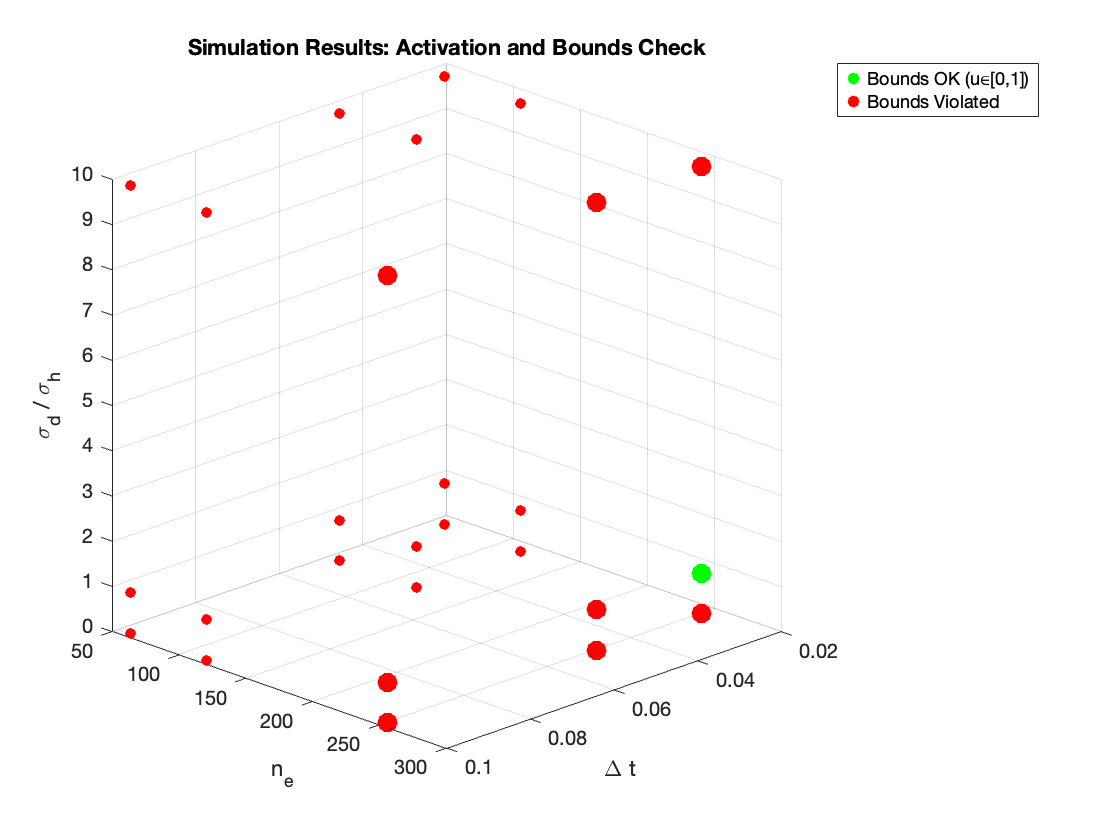
\includegraphics[width=0.8\textwidth]{assets/images/sim_results.png}
%     \caption{Confronto delle soluzioni per $t=20$ ottenute con diversi metodi}
%     \label{fig:sim_comparison}
% \end{figure}

Il modello DeepRitz ottimizzato ha dimostrato:
\begin{itemize}
    \item Maggiore regolarità rispetto alla soluzione FEM
    \item Migliore riproduzione dell'interfaccia tra regioni a diversa diffusività rispetto alle PINN
    \item Capacità di generalizzare a parametri fisici non visti durante l'addestramento, a differenza delle CNN
\end{itemize}

\subsection{Lezioni apprese e conclusioni}

Il nostro processo di fine-tuning del modello DeepRitz ha evidenziato diversi principi chiave:

\begin{itemize}
    \item \textbf{L'importanza della regolarità}: La sostituzione della condizione iniziale a gradino con una gaussiana ha mostrato quanto sia cruciale avere funzioni regolari per l'addestramento di reti neurali.
    
    \item \textbf{Il bilanciamento delle componenti della loss}: L'assegnazione di pesi appropriati alle diverse componenti della funzione obiettivo è essenziale per guidare l'apprendimento verso soluzioni fisicamente accurate.
    
    \item \textbf{La generalizzazione attraverso campionamento dinamico}: La rigenerazione dei punti di collocazione ad ogni epoca è stata determinante per ottenere un modello robusto che generalizza bene su tutto il dominio.
    
    \item \textbf{La continuità nel processo di ottimizzazione}: L'implementazione di un sistema di checkpointing completo ha permesso sessioni di addestramento incrementali senza perdita di informazioni.
    
    \item \textbf{La necessità di capacità rappresentativa}: Un'architettura sufficientemente profonda e larga si è rivelata indispensabile per catturare le complesse dinamiche spazio-temporali dell'equazione del monodominio.
\end{itemize}

In conclusione, il nostro lavoro ha dimostrato che, attraverso un processo sistematico di ottimizzazione, i metodi basati su reti neurali come DeepRitz possono produrre soluzioni competitive con i metodi numerici tradizionali per problemi complessi come l'equazione del monodominio, offrendo al contempo maggiore flessibilità e adattabilità a diverse condizioni fisiche.

% \begin{figure}[H]
%     \centering
%     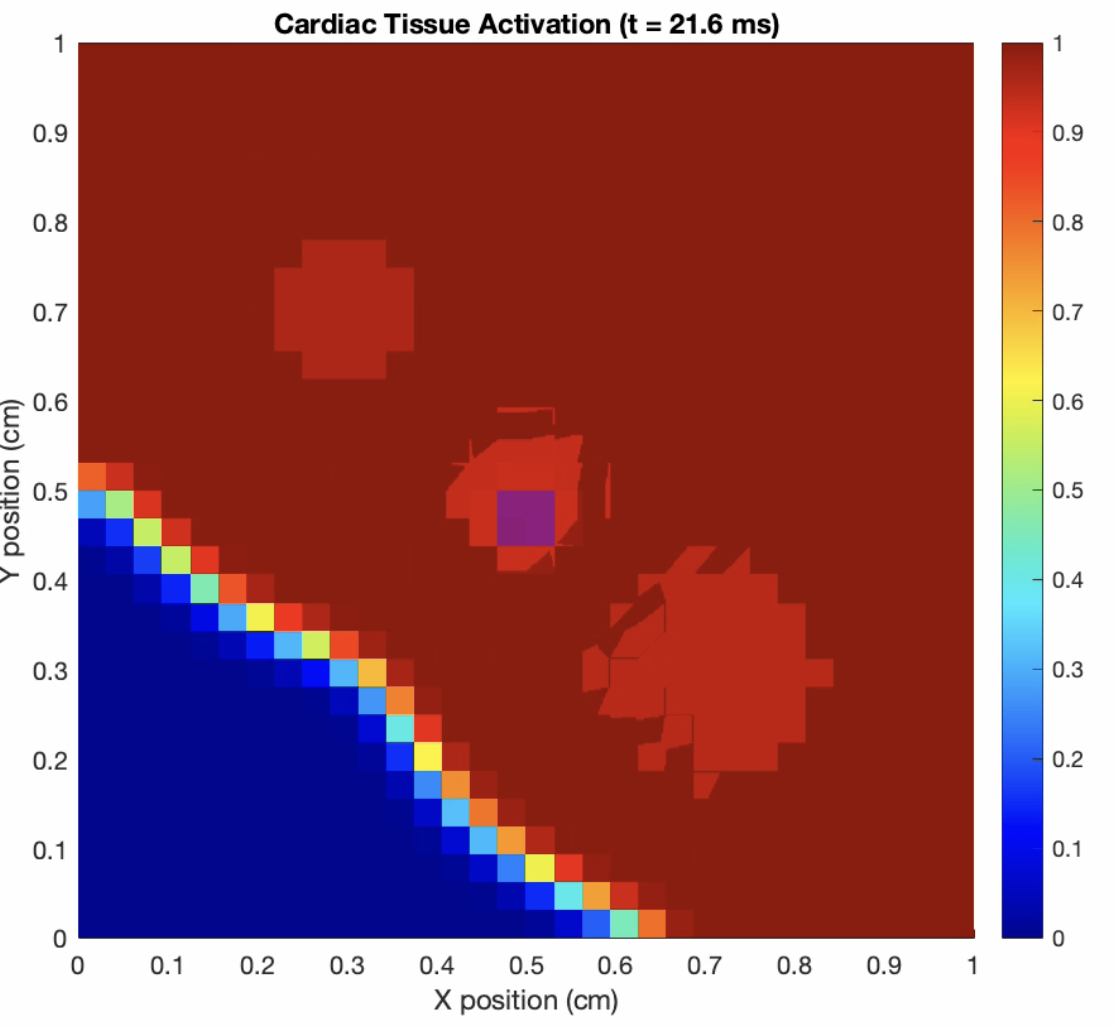
\includegraphics[width=0.8\textwidth]{assets/images/activation_t21.png}
%     \caption{Propagazione dell'onda cardiaca al tempo $t=21$ con il modello DeepRitz ottimizzato, che mostra chiaramente l'influenza delle regioni a diversa diffusività}
%     \label{fig:wave_propagation}
% \end{figure}
